\documentclass[12pt, twoside]{book}
%\documentclass[12pt, oneside]{book}  % single-sided printing

% correct margin setting
\usepackage[a4paper,top=2.5cm,bottom=2.5cm,left=3.5cm,right=2cm]{geometry}
% enabling fonts for UTF8 encoding
\usepackage[utf8]{inputenc}
\usepackage[T1]{fontenc}

% setting line spacing according to the directive
\linespread{1.25} % a value of 1.25 should correspond to 1.5 line spacing

% package for better display of references
\usepackage[backend=biber]{biblatex}
\addbibresource{references.bib}

% package for advanced color usage
\usepackage{xcolor}

\definecolor{background}{rgb}{0.95,0.95,0.95}
\definecolor{placeholder}{rgb}{0.07,0.04,0.56}
\definecolor{string}{rgb}{0.0,0.5,0.0}
\definecolor{highlight}{rgb}{0.8,0.0,0.0}
\definecolor{comment}{rgb}{0.66, 0.66, 0.66}

% package for inserting images
\usepackage{graphicx}

% package for inserting entire pdf documents (thesis assignment)
\usepackage{pdfpages}

% package for properly formatting URLs
\usepackage{url}
% package for hyperlinks within the document (we will remove the colored frames around the lines so that the pdf looks the same as the printed version)
\usepackage[hidelinks,breaklinks]{hyperref}

\usepackage{cleveref}
\crefname{lstlisting}{command}{commands}
\crefname{table}{list}{lists}

\usepackage{tikz}

% package for adjustwidth environment
\usepackage{changepage}

% idk
\usepackage{fancyvrb}

% package for importing source code
\usepackage{listings}

\usepackage{caption}

% package for proper functioning of the figure [H] environment
\usepackage{float}

% package for large tables
\usepackage{longtable}

\newcommand{\TODO}[1]{\textcolor{blue}{TODO -- #1}}

\newcommand{\shell}{\textcolor{placeholder}{\texttt{$\langle$SHELL$\rangle$}}}
\newcommand{\host}{\textcolor{placeholder}{\texttt{$\langle$HOST$\rangle$}}}
\newcommand{\port}{\textcolor{placeholder}{\texttt{$\langle$PORT$\rangle$}}}
\newcommand{\portt}{\textcolor{placeholder}{\texttt{$\langle$PORT2$\rangle$}}}
\newcommand{\tmp}{\textcolor{placeholder}{\texttt{$\langle$TMP$\rangle$}}}
\newcommand{\script}{\textcolor{placeholder}{\texttt{$\langle$compressed-script$\rangle$}}}

\newcommand{\inlinecmdline}[1]{\colorbox{background}{\texttt{#1}}}

\newcommand{\cmdlstsettings}[4]
{\lstset{
	language={#1},
	otherkeywords={#3},
	morekeywords=[1]{#3},
	morekeywords=[2]{#4},
	basicstyle={\ttfamily\footnotesize},
	backgroundcolor={\color{background}},
	commentstyle={\color{comment}},
	stringstyle={\color{string}},
	keywordstyle={\color{highlight}},
	keywordstyle=[2]{\color{blue}},
	showspaces=false,
	showstringspaces=false,
	columns=fullflexible,
	breaklines=true,
	escapechar={#2},
	frame=single,
	rulecolor={\color{black}},
	framesep=5pt,
	framerule=0.8pt
}}

\newenvironment{cmdline}[4]
{\begingroup
\cmdlstsettings{#1}{#2}{#3}{#4}
\VerbatimOut{tmp.txt}}
{\endVerbatimOut
\lstinputlisting{tmp.txt}
\endgroup}

\newcommand{\getcmdline}[7]{\begingroup
\cmdlstsettings{#2}{#3}{#4}{#5}
\lstinputlisting[label={lst:#7},caption={#6}]{#1}
\endgroup}

\renewcommand{\lstlistingname}{Command}

\setlength{\parindent}{0pt}
\setlength{\parskip}{6pt}


\def\mfrok{2025}
\def\mfnazov{Analysis of reverse shell techniques and possible countermeasures}
\def\mftyp{Bachelor Thesis}
\def\mfautor{Matúš Bucher}
\def\mfskolitel{Ing. Dušan Bernát, PhD.}

\def\mfmiesto{Bratislava, \mfrok}

\def\mfodbor{Computer Science}
\def\program{Computer Science }

\def\mfpracovisko{ Department of Computer Science }

\begin{document}
\frontmatter
\pagestyle{empty}

% -------------------
% --- Obalka ------
% -------------------

\begin{center}
  \sc\large
  Comenius University in Bratislava\\
  Faculty of Mathematics, Physics and Informatics

\vfill

{\LARGE\mfnazov}\\
\mftyp
\end{center}

\vfill

{\sc\large 
\noindent \mfrok\\
\mfautor
}

\cleardoublepage
% --- koniec obalky ----

% -------------------
% --- Titulný list
% -------------------

\noindent

\begin{center}
\sc  
\large
  Comenius University in Bratislava\\
  Faculty of Mathematics, Physics and Informatics

\vfill

{\LARGE\mfnazov}\\
\mftyp
\end{center}

\vfill

\noindent
\begin{tabular}{ll}
Study Programme: & \program \\
Field of Study: & \mfodbor \\
Department: & \mfpracovisko \\
Supervisor: & \mfskolitel \\
\end{tabular}

\vfill


\noindent \mfmiesto\\
\mfautor

\cleardoublepage
% --- Koniec titulnej strany


% -------------------
% --- Zadanie z AIS
% -------------------
% v tlačenej verzii s podpismi zainteresovaných osôb.
% v elektronickej verzii sa zverejňuje zadanie bez podpisov
% v pracach v anglictine anglicke aj slovenske zadanie

\newpage
\setcounter{page}{3}
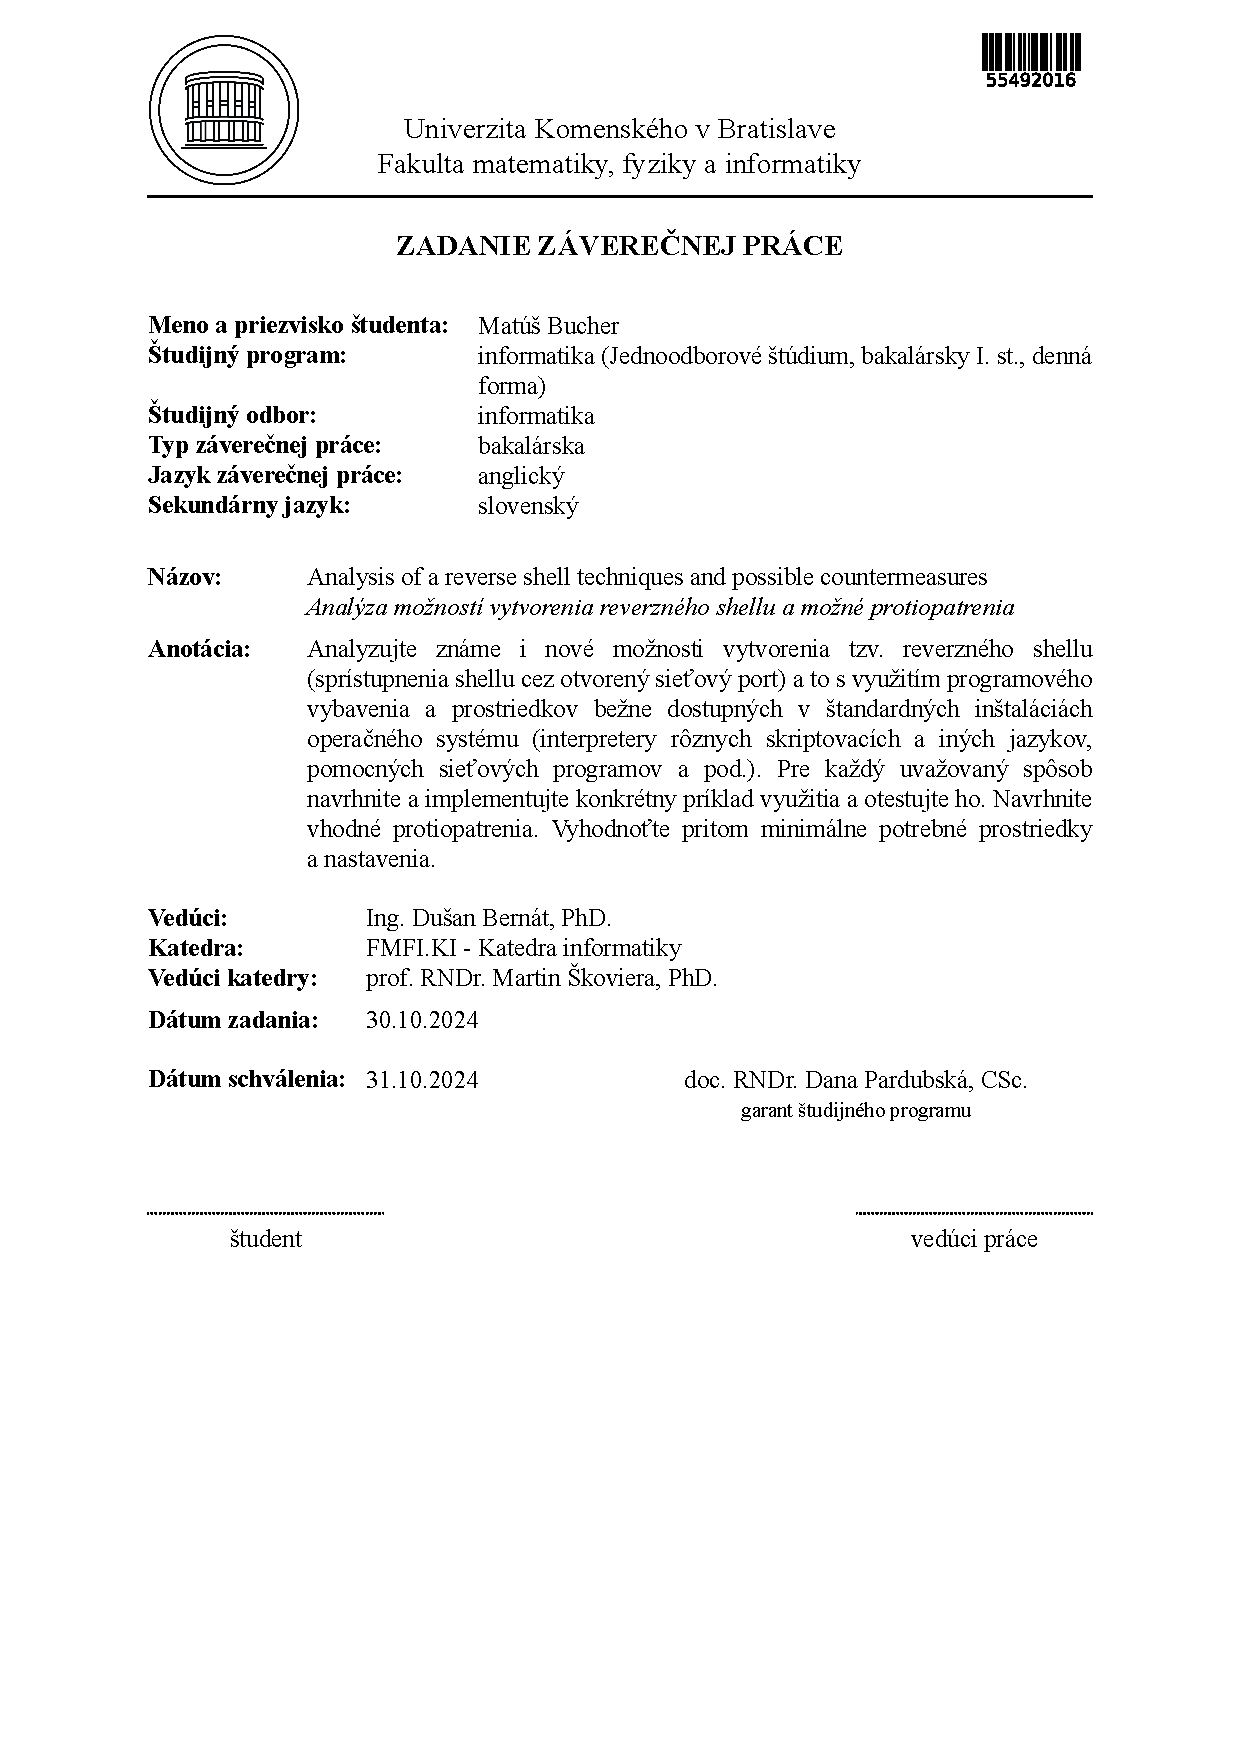
\includepdf{images/zadanie.pdf}

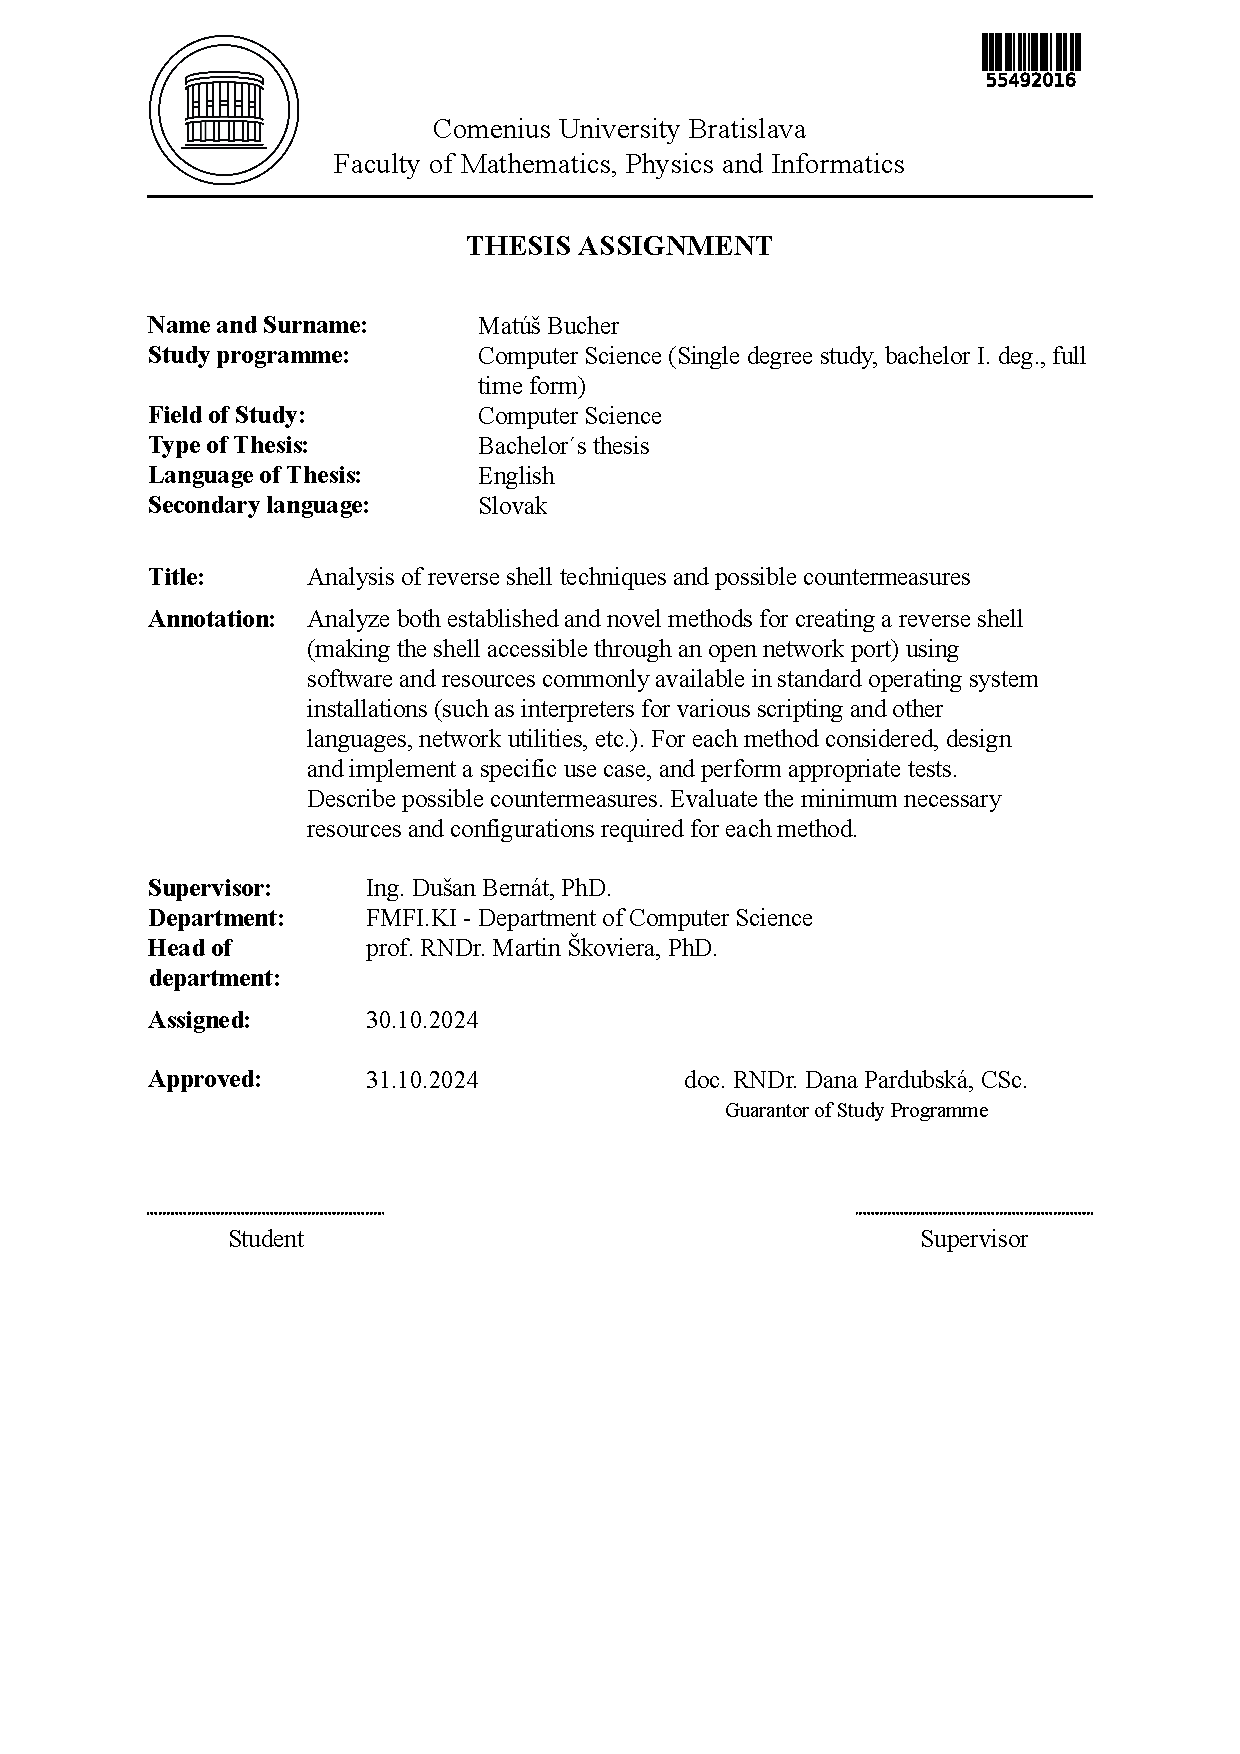
\includepdf{images/zadanie-en.pdf}

% --- Koniec zadania


% -------------------
%   Poďakovanie - nepovinné
% -------------------
\newpage
\pagestyle{plain}
~

\vfill
{\bf Acknowledgments:} \TODO{add acknowledgments}

% --- Koniec poďakovania

% -------------------
%   Abstrakt - Slovensky
% -------------------
\newpage
\section*{Abstrakt}


\TODO{add abstract in Slovak}

\paragraph*{Kľúčové slová:} \TODO{add keywords in Slovak}
% --- Koniec Abstrakt - Slovensky


% -------------------
% --- Abstrakt - Anglicky 
% -------------------
\newpage 
\section*{Abstract}

\TODO{add abstract in English}


\paragraph*{Keywords:} \TODO{add keywords in English}

% --- Koniec Abstrakt - Anglicky

% -------------------
% --- Predhovor - v informatike sa zvacsa nepouziva
% -------------------
%\newpage 
%
%
%\chapter*{Preface} %
%
%Predhovor je všeobecná informácia o práci, obsahuje hlavnú charakteristiku práce 
%a okolnosti jej vzniku. Autor zdôvodní výber témy, stručne informuje o cieľoch 
%a význame práce, spomenie domáci a zahraničný kontext, komu je práca určená, 
%použité metódy, stav poznania; autor stručne charakterizuje svoj prístup a svoje
%hľadisko. 
%
% --- Koniec Predhovor


% -------------------
% --- Obsah
% -------------------

\cleardoublepage 

\tableofcontents

% ---  Koniec Obsahu

% -------------------
% --- Zoznamy tabuliek, obrázkov - nepovinne
% -------------------

\newpage 

\listoffigures
\listoftables

% ---  Koniec Zoznamov

\mainmatter
\pagestyle{headings}

\input intro.tex 

\input chapters/chapter1/chapter1.tex

\input chapters/chapter2/chapter2.tex

\input chapters/chapter3/chapter3.tex

\input chapters/chapter4/chapter4.tex

\input conclusion.tex



%\input zaver.tex

% -------------------
% --- Bibliografia
% -------------------


\newpage	

\backmatter

\thispagestyle{empty}
\clearpage

\printbibliography 

%---koniec Referencii

% -------------------
%--- Prilohy---
% -------------------

\input appendix.tex

\end{document}
